\section{Introduction}\label{sec:intro}


A central goal of machine learning research is to develop unified architectures capable of learning and reasoning across a wide range of tasks and data modalities. However, there is a tension between the goal of creating a general architecture and the need to support inductive biases that are beneficial for certain types of tasks~\citep{wolpert1995no,baxter2000model}. With a finite training set and multiple possible solutions for empirical risk minimization, inductive biases guide the learning algorithm to prioritize solutions with specific properties, thereby enabling greater data efficiency and improved generalization to new inputs. A tantalizing hypothesis is that human and animal intelligence can be explained by a small set of fundamental principles~\citep{marcus2003algebraic}. In the context of machine intelligence, our goal is to uncover a complete set of fundamental inductive biases with broad applicability to real-world tasks that enable robust, flexible, and data-efficient learning.

Such a unified architecture must be capable of handling general inputs of various modalities and must possess computational mechanisms for routing and processing both the attributes of objects in the input and the relations between them. In analogy to neural systems in the brain~\citep{newman1997neural}, we refer to the former as \textit{sensory} information and the latter as \textit{relational} information.

The Transformer architecture~\citep{vaswani2017attention} provides a promising candidate for the basis of a versatile general-purpose architecture for machine learning. By operating over sets or sequences of objects, Transformers are able to support highly-general inputs and outputs. More importantly, neural attention provides an effective computational mechanism for routing sensory information between different elements in the input, enabling iterative contextual processing. This has lead to remarkable empirical success across several domains, including language~\citep{kaplan2020scalinglawsneurallanguage} and visual processing~\citep{dosovitskiyImageWorth16x162020}.

Yet, recent work on relational learning has shown that Transformers struggle to efficiently learn tasks involving relational reasoning, prompting several proposals for neural architectures that incorporate inductive biases for relational learning~\citep{santoroSimpleNeuralNetwork2017,santoroRelationalRecurrentNeural2018,shanahanExplicitlyRelationalNeurala,webbEmergentSymbolsBinding2021,webbRelationalBottleneckInductive2024,kergNeuralArchitectureInductive2022,altabaa2024abstractors,altabaaLearningHierarchicalRelational2024}. Relational reasoning is an essential component of general intelligence, making the lack of support for efficient and robust relational learning a fundamental limitation of the Transformer framework. The ultimate power of relational reasoning lies in its capacity to to generate inferences and generalizations in systematic and novel ways, which, in the limit, can lead to universal inductive generalization from a small set of observations to a potential infinite set of novel instances~\citep{goyal2022inductive}.

In this paper, we posit the following explanation for the Transformer's limited abilities in relational learning: while neural attention provides a powerful mechanism for routing \textit{sensory} information between objects in the input, the Transformer lacks an explicit computational mechanism for routing and processing \textit{relational} information between objects. Thus, we argue that standard Transformers possess an incomplete set of inductive biases, notably lacking inductive biases for relational learning. The goal of this paper is to propose an extension of the Transformer framework which enables explicit routing and processing of both sensory and relational information.

To understand our proposed method at a high-level, it can be useful to view standard Transformers as an instantiation of a broader neural message-passing computational paradigm that consists of iterative information retrieval followed by local processing. In its general form, a collection of objects $x_1,\ldots, x_n$ are processed via an iterative application of
\begin{equation}\label{eq:intro_message_passing}
  \begin{split}
    x_i &\gets \mathrm{Aggregate}\bigparen{x_i, \set{m_{j \to i}}_{j=1}^{n}}, \\
    x_i &\gets \mathrm{Process}(x_i).
  \end{split}
\end{equation}
In the case of Transformers, the self-attention mechanism can be seen as sending messages from object $j$ to object $i$ that are encodings of the sender's \textit{sensory} features, with the message from sender $j$ to receiver $i$ given by $m_{j \to i} = \phi_v(x_j)$. These messages are then aggregated according to some selection criterion based on the receiver's features,  typically determined by softmax attention scores. 

To enable explicit relational representation learning, we propose a novel attention mechanism that attends over and routes the relational information between objects in the input. In \textit{relational attention}, the message from the sender object to the receiver object is a set of relations between them, which can be expressed as $m_{j \to i} = r(x_i, x_j)$. Here, the relation $r(\cdot, \cdot)$ models a series of comparisons between objects across different feature dimensions dimensions via inner products of feature maps. We combine this with the standard attention mechanism of of Transformers yielding a variant of multi-head attention for processing both sensory and relational information. This \textit{Dual Attention} architecture disentangles the two types of information in the aggregation phase of attention, while integrating them during the information processing stage.

The contributions in this paper are summarized as follows:
\begin{enumerate}
  \item We introduce a new \textit{relational attention} mechanism that disentangles sensory information from relational information. While standard self-attention models retrieval of sensory information, relational attention models retrieval of relational information.
  \item We introduce a generalized Transformer architecture that integrates sensory and relational information through \textit{Dual Attention}---a form of multi-head attention with two distinct types of attention heads. Standard self-attention heads encode sensory information, while relational attention heads encode relational information.
  \item We carry out a thorough and diverse set of experiments, showing that the \textit{Dual Attention Transformer} outperforms standard Transformers in terms of data efficiency across a range of tasks, suggesting that relational inductive biases are an important component of the general machine intelligence and learning systems we seek.
\end{enumerate}

\begin{figure}[t]
  \centering
  \begin{subfigure}[t]{0.415384615\textwidth} % 0.9 * 3 / 6.5
    \centering
    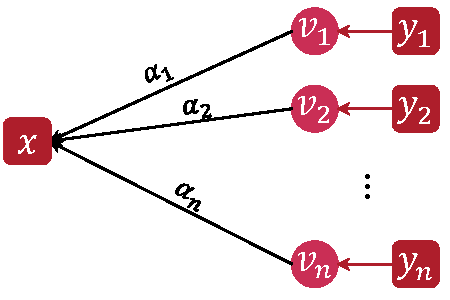
\includegraphics[width=\textwidth]{figs/sensory_retrieval.pdf} % size: 3 x 2 in
    \caption{$\Attn(x, \ys)$}%: Retrieval of sensory information by standard attention.}
  \end{subfigure}
  \qquad
  \begin{subfigure}[t]{0.484615385\textwidth} % 0.9 * 3.5 / 6.5
    \centering
    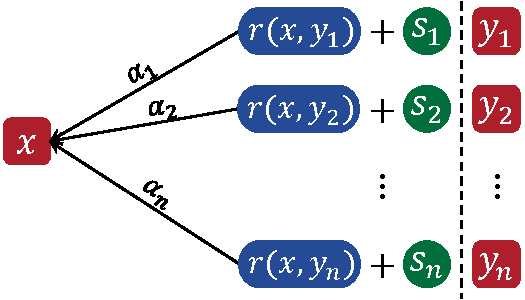
\includegraphics[width=\textwidth]{figs/relational_retrieval.pdf} % size 3.5 x 2 in
    \caption{$\RelAttn(x, \ys)$}%: Retrieval of relational information by relational attention.}
  \end{subfigure}
  % 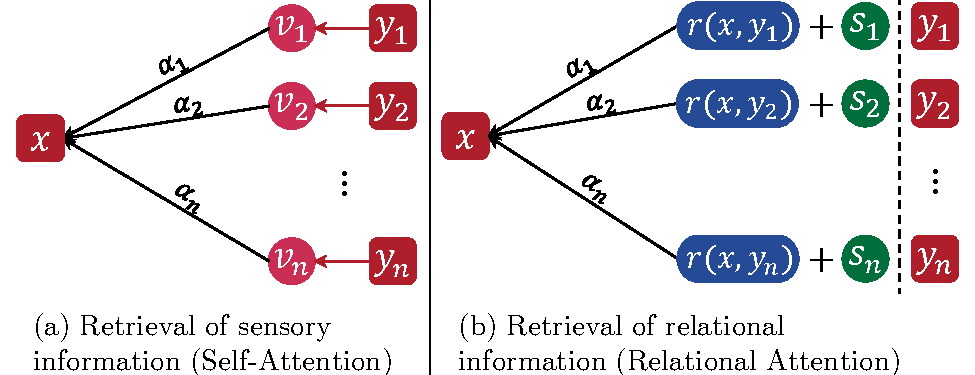
\includegraphics[width=0.8\textwidth]{figs/attn_fig_combined_noqeuerykey.pdf}
  \caption{Standard self-attention retrieves sensory information $v_i$ about the attributes of individual objects while \textit{relational attention} retrieves relational information $r(x, y_i)$ about the relationship between the objects in the context and the receiver.
  Each relation is tagged with a symbol $s_i$ which acts as an abstract variable identifying the sender.
  In both cases, information is aggregated according to the attention scores $\alpha_i$, which are computed by a softmax over inner products of queries and keys.
  }\label{fig:selfattn_relattn}
  \vskip-7pt
\end{figure}